\section{Hyperparameters and training details}
\label{sec:appendix-hyper}

This appendix collects the hyperparameters used for every method
in \Cref{sec:experiments}. All numbers are the configuration that
generated the headline tables in \Cref{sec:results}.

\paragraph{Shared LC-PINN configuration.}
Network: 4-layer MLP, hidden widths $[64, 64, 64, 64]$, $\tanh$
activations, Xavier initialisation. Conditioning route is
mode-dependent: concat at the input layer for the loss-weight mode
(Burgers, BL); FiLM \citep{perez2018film} on every hidden layer
followed by an L-BFGS finishing pass with a revert-on-worse safety
check for the parametric-coefficient mode (Helmholtz, Schrödinger).
Optimiser: Adam,
$\eta\!=\!10^{-3}$, cosine-annealed to $10^{-5}$ over the full
budget, gradient clip $1.0$. Mini-batch composition: $n_\lambda\!=\!4$
parameter samples per step, each with the per-equation collocation
counts below. Backend: PyTorch~2.9 with the MPS device on a single
Apple~M4 Max.

\paragraph{Per-equation collocation and budgets.}
\Cref{tab:hyper-lc} lists the LC-PINN collocation counts and step
budgets per PDE family.

\begin{table}[h]
\centering
\caption{LC-PINN collocation counts and step budgets per PDE family.}
\label{tab:hyper-lc}
\begin{tabular}{lcccc}
\toprule
PDE & interior & boundary & initial & Adam / L-BFGS \\
\midrule
Burgers           & $1024$ & $200$ & $200$ & $50\text{k}\,/\,0$    \\
BL (viscous)      & $1024$ & $200$ & $200$ & $50\text{k}\,/\,0$    \\
Helmholtz (1D)    & $1024$ & $100$ & ---   & $50\text{k}\,/\,1.5\text{k}$ \\
Helmholtz (2D)    & $4096$ & $400$ & ---   & $25\text{k}\,/\,1.5\text{k}$ \\
Helmholtz (3D)    & $8192$ & $600$  & ---  & $25\text{k}\,/\,1.5\text{k}$ \\
Schrödinger (1D)  & $1024$ & $64$  & ---   & $50\text{k}\,/\,1.5\text{k}$ \\
\bottomrule
\end{tabular}
\end{table}

\paragraph{Baseline configurations.}
All single-$\lambda$ baselines share the LC-PINN backbone (same
widths, activation, initialisation, and Adam schedule) so that the
amortisation comparison is on equal architectural footing.

\begin{itemize}\setlength{\itemsep}{0pt}
\item \emph{SA-PINN \citep{mcclenny2020}}: per-collocation-point
      trainable weight ascended on the residual; Adam phase
      $10\text{k}$ iterations, then weights frozen and L-BFGS phase
      $5\text{k}$ iterations on the unweighted loss.
\item \emph{ReLoBRaLo \citep{bischof2021}}: 3-term loss-weight
      balancer (residual / boundary / initial) with softmax over
      log-loss-ratios, smoothed by EMA. Hyperparameters
      $\alpha\!=\!0.999$, $\tau\!=\!0.1$,
      $\rho_{\text{mean}}\!=\!0.999$.
\item \emph{Causal-PINN \citep{wang2024}}: time-causal residual mask
      $w(t)\!=\!\exp\!\left(-\varepsilon\,R(<\!t)\right)$ with
      $\varepsilon\!=\!100$. Burgers and BL only.
\item \emph{PI-DeepONet \citep{wang2021pi-deeponet}}: branch--trunk
      architecture; branch encodes the wavenumber $k$ via a 4-layer
      MLP (hidden width $128$); trunk encodes the spatial coordinate
      $x$ via a 4-layer MLP (hidden width $128$). Final solution is
      the inner product of branch and trunk outputs. Loss is the
      Helmholtz residual on the same collocation grid as the per-$k$
      LC-PINN, summed over an $n_k$-grid of branch inputs ($n_k\!=\!20$).
      Adam phase $50$k iterations followed by L-BFGS phase $1.5$k
      iterations with a revert-on-worse safety check; on 1D Helmholtz
      one seed (seed 1) diverged in L-BFGS and was reverted to the
      Adam-phase weights, reported as such in the 5-seed mean of
      \Cref{tab:helmholtz}.
\item \emph{FNO \citep{li2020fno}}: width $64$, $64$ Fourier modes,
      $4$ \texttt{SpectralConv1d}~+~\texttt{Conv1d}-shortcut blocks
      ($\sim\!1.07$M parameters). Optimiser: Adam,
      $\eta\!=\!10^{-3}$, weight decay~$10^{-4}$, \texttt{StepLR}
      with step~$=\!\text{epochs}/5$ and $\gamma\!=\!0.5$. Loss:
      per-sample rel-$L^2$. Training set: $512$ random Fourier
      initial conditions (truncated 6-mode spectrum, decaying
      amplitude) solved by the same Radau scheme used for the
      reference; $2000$ epochs.
\end{itemize}

\paragraph{Reference solutions.}
Burgers reference: Fourier-spectral spatial discretisation with a
Radau IIA implicit time integrator, integrated to relative residual
$<\!10^{-6}$ on a $512\!\times\!1001$ space--time grid.
Buckley--Leverett reference: explicit Lax--Friedrichs flux on
$n_x\!=\!1000$ with centred-difference viscous regularisation,
CFL-limited time stepping. Helmholtz~1D reference: closed-form
manufactured solution $u(x;k)\!=\!\sin(\pi x)\cos(kx)$ with the
forcing $f$ chosen to match. Helmholtz~2D reference: closed-form
manufactured solution
$u(x,y;k) \!=\! \sin(\pi x)\sin(\pi y)\cos(kx)\cos(ky)$. Letting
$a(x;k)\!=\!\sin(\pi x)\cos(kx)$ and
$b(y;k)\!=\!\sin(\pi y)\cos(ky)$, so $u\!=\!a(x;k)\,b(y;k)$, the
forcing
\[
   f(x,y;k) \;=\; \Delta u + k^2 u
   \;=\; -\bigl(2\pi^2 + k^2\bigr)\, u
         \;-\; 2\pi k\,\bigl[\cos(\pi x)\sin(kx)\sin(\pi y)\cos(ky) +
                              \sin(\pi x)\cos(kx)\cos(\pi y)\sin(ky)\bigr]
\]
agrees with a centred-difference numerical Laplacian on the
manufactured solution to absolute error $<\!4\!\times\!10^{-6}$.
Helmholtz~3D reference: closed-form manufactured solution
$u(x,y,z;k)\!=\!\sin(\pi x)\sin(\pi y)\sin(\pi z)\cos(kx)\cos(ky)\cos(kz)$
on the unit cube, with the matching forcing
$f \!=\! \Delta u + k^2 u$ derived analytically; agreement to a
centred-difference numerical Laplacian is $<\!10^{-5}$ across
$k\!\in\!\{1,3,5\}$. Schrödinger reference: with $u(x;\alpha)\!=\!\sin(\pi x)\,g(x;\alpha)$,
$g(x;\alpha)\!=\!e^{-\alpha (x-1/2)^2/2}$, the forcing is
\[
   f(x;\alpha) \;=\; -u'' + V(x;\alpha)\, u
   \;=\; (\pi^2 + \alpha)\, u
         \;+\; 2\pi\alpha\,(x-\tfrac12)\,\cos(\pi x)\, g(x;\alpha),
\]
which agrees with a centred-difference numerical residual to
$<\!5\!\times\!10^{-6}$ across $\alpha\in\{0.5,2,5,10\}$.

\paragraph{Evaluation grids.}
Burgers / BL test errors are computed on a $256\!\times\!101$
space--time grid; Helmholtz on a $1024$-point spatial grid. The
$K$-shot averaged LC-PINN prediction is the mean of $K$ forward
passes at independent $\lambda$ samples from $p_\lambda$; we use
$K\!=\!100$ for Burgers and $K\!=\!25$ for BL in the headline
tables.

\paragraph{Compute.}
Each run uses a single Apple~M4~Max with the PyTorch MPS backend.
Reported wall times are end-to-end per seed (model construction,
training, and evaluation), measured with \texttt{time.perf\_counter}.

\paragraph{Reproducibility.}
Random seeds: $\{0, 1, 2, 3\}$ for the four headline replicates;
$\{0, 1\}$ for the 2-seed ablation budgets. Each seed controls the
PyTorch global RNG and the NumPy RNG used to draw collocation
points and $\lambda$-samples. The full training script, equation
modules, and reference solvers are released with the
camera-ready version.

\section{Ablations: full protocol and numbers}
\label{sec:appendix-ablations}

\paragraph{$K$-shot averaging.}
Sweeping $K \in \{25, 50, 100, 200, 400\}$ on the trained LC-PINN
gives essentially constant rel-$L^2$ ($3.51\!\times\!10^{-3}$ at
$K\!=\!25$, $3.49\!\times\!10^{-3}$ at $K\!=\!100$,
$3.49\!\times\!10^{-3}$ at $K\!=\!400$; spread
$\pm 2.7\!\times\!10^{-3}$ stays roughly constant). At the optimum
each $\lambda$-slice is already a residual minimiser
(Proposition~1), so increasing $K$ adds samples but no new
information.

\paragraph{$n_\lambda$ per training step.}
At a matched 25k-epoch budget on Burgers (2 seeds), sweeping
$n_\lambda \!\in\! \{1, 4, 16\}$ per step gives non-monotone
behaviour: $n_\lambda\!=\!1\!\to\!1.69\!\times\!10^{-2}$,
$n_\lambda\!=\!4\!\to\!1.22\!\times\!10^{-2}$,
$n_\lambda\!=\!16\!\to\!1.50\!\times\!10^{-1}$. Too few
$\lambda$ per step makes the gradient estimate of the
$p_\lambda$-expectation noisy (Remark~3 / Hoeffding); too many
concentrates compute into fewer optimisation steps and the network
does not converge in the fixed budget. At the headline 50k-epoch
budget we use $n_\lambda\!=\!4$.

\paragraph{Sampling distribution $p_\lambda$.}
At matched 25k-epoch / $n_\lambda\!=\!4$ / 2-seed budget on
Burgers, swapping $p_\lambda$ from uniform on the simplex to
log-uniform gives rel-$L^2$ of
$1.22\!\times\!10^{-2} \pm 5.14\!\times\!10^{-3}$ (uniform) versus
$1.74\!\times\!10^{-1} \pm 9.26\!\times\!10^{-3}$ (log-uniform), a
$\sim\!14\times$ degradation. We read this not as a contradiction
with Remark~2 (an asymptotic-optimum statement) but as a
finite-budget effect: log-uniform places dominant mass on small
loss weights, weakening the gradient signal at large $\lambda$
values where the residual contributes most to the test-relevant
slices.

\section{FiLM does not help in loss-weight mode}
\label{sec:appendix-film-loss-weight}

In the parametric-coefficient mode (Helmholtz, Schrödinger) FiLM
modulation lifts the LC-PINN by an order of magnitude: on 1D
Helmholtz, plain concat reaches rel-$L^2 \!\sim\!9\!\times\!10^{-3}$
on the same $k$-grid (\texttt{lc\_pinn\_helmholtz} runs), whereas
FiLM$+$L-BFGS reaches $9.4\!\times\!10^{-4}$ (\Cref{tab:helmholtz},
$\sim\!10\times$ tighter). In the loss-weight mode (Burgers) it
regresses: a four-seed re-run of Burgers with
FiLM$+$L-BFGS gave $5.7\!\times\!10^{-2} \pm 5.5\!\times\!10^{-2}$,
with two seeds at the concat baseline ($\sim\!3\!\times\!10^{-3}$)
and two trapped near $10^{-1}$. We read this as evidence that
FiLM's value lies in disentangling \emph{operator}-changing inputs
from spatial coordinates; loss-weight inputs do not change the
operator, so FiLM gates over a degree of freedom that does not
exist. The headline Burgers and BL rows in
\Cref{sec:results-burgers-bl} therefore use the simpler
concat$+$Adam configuration of \citet{dosovitskiy2020}.

\section{Per-parameter breakdowns}
\label{sec:appendix-per-param}

The per-$\alpha$ breakdown for 1D Schrödinger
(\Cref{sec:results-schrodinger}) is given in
\Cref{tab:schrod-per-alpha}.

\begin{table}[h]
\centering
\caption{Per-$\alpha$ rel-$L^2$ on 1D parametric Schrödinger
(mean $\pm$ std over 4 LC seeds and 2 SA seeds per $\alpha$).
Bold: best per row.}
\label{tab:schrod-per-alpha}
\small
\begin{tabular}{r|cc}
\toprule
$\alpha$ & SA-PINN (per-$\alpha$) & LC-PINN (one net) \\
\midrule
$0.5$  & $\mathbf{(5.89\!\pm\!1.26)\!\times\!10^{-5}}$ & $(3.69\!\pm\!3.23)\!\times\!10^{-4}$ \\
$5.0$  & $(1.07\!\pm\!1.05)\!\times\!10^{-2}$ & $\mathbf{(7.50\!\pm\!4.25)\!\times\!10^{-5}}$ \\
$10.0$ & $(9.29\!\pm\!6.67)\!\times\!10^{-4}$ & $\mathbf{(1.54\!\pm\!0.72)\!\times\!10^{-4}}$ \\
\midrule
\textbf{grid mean} & $3.89\!\times\!10^{-3}$ & $\mathbf{1.99\!\times\!10^{-4}}$ \\
\bottomrule
\end{tabular}
\end{table}

\Cref{fig:per_alpha_schrodinger} visualises the same data on the
20-point LC/DON grid alongside SA's 3 training points. The two
amortised methods (LC and DON) hold a flat $\sim\!10^{-4}$ curve
across the entire $\alpha\in[0.5,10]$ range; the per-$\alpha$
SA-PINN baseline matches at $\alpha=0.5$ and $\alpha=10$ but
collapses by two orders of magnitude at the intermediate
$\alpha=5.0$ training point --- the same incoherence pattern
documented for Helmholtz in \Cref{sec:results-helmholtz}.

\begin{figure}[h]
\centering
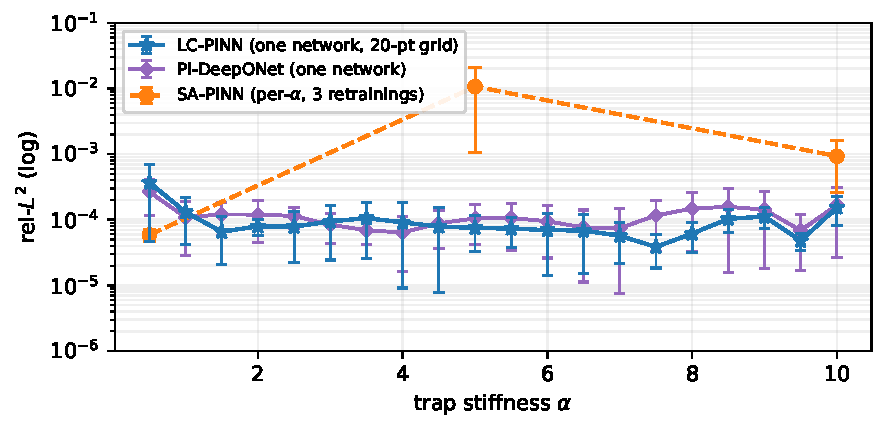
\includegraphics[width=0.75\linewidth]{figures/per_alpha_schrodinger.pdf}
\caption{Per-$\alpha$ rel-$L^2$ on 1D parametric Schrödinger.
LC-PINN (blue, 4 seeds) and PI-DeepONet (purple, 4 seeds) cover the
20-point grid from one trained network each; SA-PINN (orange, 2
seeds) is three separate retrainings at $\alpha\in\{0.5,5.0,10.0\}$.
Error bars are $\pm$std on a log axis.}
\label{fig:per_alpha_schrodinger}
\end{figure}
